\chapter{열린 끈의 양자에서 타키온과 중력까지}

\lectureoverview{이제 지난 강의에서 구한 정상 모드를 양자화하고, 그 결과 어떤 입자 상태가 만들어지는지 살펴보자. 각 횡방향 모드는 조화 진동자이지만, 정규화 방식은 다소 낯설다. \(n\) 모드를 들뜨게 하면 광전면 에너지가, 따라서 질량제곱 준위가 \(n\)만큼 증가한다. 열린 끈의 첫 번째 들뜬 준위는 질량이 없는 벡터의 두 횡방향 편광과 정확히 같은 방식으로 변환한다. 그러므로 상대론적 일관성을 만족하려면 바닥 상태의 질량제곱은 음수여야 한다. 이 상태가 보손 끈의 타키온이다. 타키온의 실제 의미는 현실적으로 빛보다 빠르게 움직이는 입자가 아니라 불안정한 진공이다. 마지막으로 끈이 상호작용하면 끈의 결합과 분리 때문에 닫힌 끈을 피할 수 없으며, 닫힌 끈의 가장 낮은 들뜸은 중력자가 된다.}

\section{각 끈 모드에 숨어 있는 진동자}

횡방향 좌표 \(X\) 하나에 대해, \(n\)번째 비영 정상 모드의 에너지와 라그랑지안은

\begin{align}
  E_n
  &=
  \frac14\dot X_n^{\,2}
  +\frac{n^2}{4}X_n^2,
  \label{eq:l03-mode-energy}\\
  L_n
  &=
  \frac14\dot X_n^{\,2}
  -\frac{n^2}{4}X_n^2.
  \label{eq:l03-mode-lagrangian}
\end{align}

\(1/4\) 인자는 오류가 아니다. 끈의 작용을 독립적인 푸리에 모드로 환원할 때 선택한 정규화가 이 인자에 반영되어 있다. 따라서 해밀토니안을 구성하는 첫 단계는 정준 운동량을 계산하는 것이다.

\begin{equation}
  p_n=\frac{\partial L_n}{\partial\dot X_n}
     =\frac12\dot X_n,
  \qquad
  \dot X_n=2p_n.
  \label{eq:l03-canonical-momentum}
\end{equation}

르장드르 변환을 하면 다음을 얻는다.

\begin{equation}
  H_n=p_n\dot X_n-L_n
     =p_n^2+\frac{n^2}{4}X_n^2.
  \label{eq:l03-mode-hamiltonian}
\end{equation}

\begin{figure}[H]\centering
  \includegraphics[width=0.82\textwidth]{lecture_03_figure_01.png}\caption{열린 끈에서 물려받은 정규화로 나타낸 모드의 에너지, 라그랑지안, 정준 운동량, 해밀토니안.}\lectureframe{00:05:40}\label{fig:l03-mode-hamiltonian-board}\end{figure}

\(H_n\)을 인수분해하려면 \(X_n\)와 \(p_n\)를 다음과 같이 결합한다.

\begin{equation}
  \frac{nX_n}{2}\pm i p_n.
\end{equation}

고전적으로는 두 인자가 교환하겠지만, 양자역학에서는 다음과 같다.

\begin{equation}
  [X_n,p_m]=i\delta_{nm}
  \label{eq:l03-canonical-commutator}
\end{equation}

\(\hbar=1\)인 단위를 사용하면 다음과 같다. 교차항들은 상쇄되어 사라지는 것이 아니다. 고정된 모드에 대해

\begin{align}
  \left[\frac{nX_n}{2}+ip_n,
        \frac{nX_n}{2}-ip_n\right]
  &=n,
  \label{eq:l03-unscaled-commutator}\\
  \left(\frac{nX_n}{2}-ip_n\right)
  \left(\frac{nX_n}{2}+ip_n\right)
  &=H_n-\frac n2.
  \label{eq:l03-factorized-hamiltonian}
\end{align}

\begin{figure}[H]\centering
  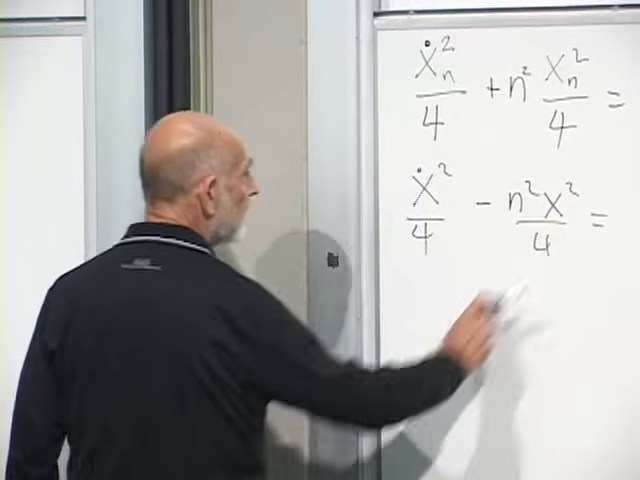
\includegraphics[width=0.82\textwidth]{lecture_03_figure_02.png}\caption{정준 교환자가 \(n\) 인자를 만들어 내는 과정을 칠판에서 계산한 모습.}\lectureframe{00:10:30}\label{fig:l03-commutator-board}\end{figure}

\(n\) 인자는 사다리 연산자를 어떻게 정규화해야 하는지 알려 준다.

\begin{align}
  a_n
  &\equiv
  \frac{\sqrt n}{2}X_n+\frac{i}{\sqrt n}p_n,
  \label{eq:l03-annihilator}\\
  a_n^\dagger
  &\equiv
  \frac{\sqrt n}{2}X_n-\frac{i}{\sqrt n}p_n.
  \label{eq:l03-creator}
\end{align}

이 연산자들은 다음 관계를 만족한다.

\begin{equation}
  [a_n,a_m^\dagger]=\delta_{nm},
  \qquad
  H_n=n\left(a_n^\dagger a_n+\frac12\right).
  \label{eq:l03-oscillator-algebra}
\end{equation}

따라서 \(a_n^\dagger\)는 \(n\)번째 진동자에 양자 하나를 더하지만, 그 양자는 모드 에너지를 \(n\)만큼 가진다. 익숙한 진동자의 에너지 간격이 사라진 것은 아니다. 그 진동수는 \(\omega_n=n\)이다.

\begin{figure}[H]\centering
  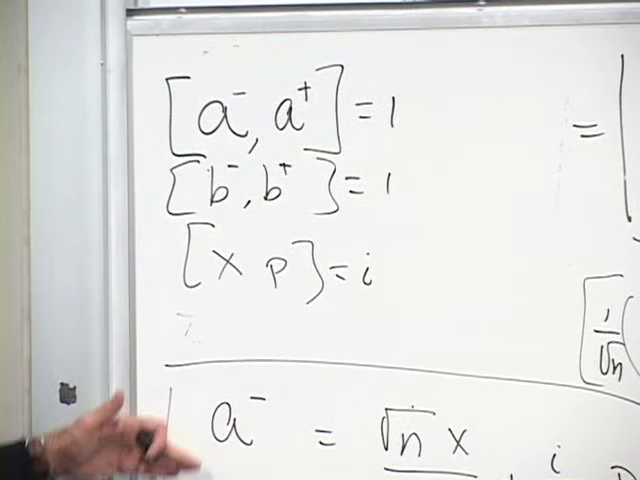
\includegraphics[width=0.82\textwidth]{lecture_03_figure_03.png}\caption{\(n\)번째 끈 진동자의 정규화된 소멸 연산자와 생성 연산자.}\lectureframe{00:12:00}\label{fig:l03-ladder-board}\end{figure}

\subsection{두 개의 횡방향 모드 계열}

시공간이 4차원일 때, \(z\)축을 따라 매우 큰 운동량을 가진 끈에는 횡방향 좌표가 두 개, \(X\)와 \(Y\)가 있다. 따라서 서로 독립적인 진동자 계열 두 개가 필요하다. \(a_n,a_n^\dagger\)는 \(X\) 모드에 작용하고, \(b_n,b_n^\dagger\)는 \(Y\) 모드에 작용한다고 하자. 좌표에 대해 \eqref{eq:l03-annihilator}--\eqref{eq:l03-creator}를 풀면 다음을 얻는다.

\begin{equation}
  X_n=\frac{a_n+a_n^\dagger}{\sqrt n},
  \qquad
  Y_n=\frac{b_n+b_n^\dagger}{\sqrt n}.
  \label{eq:l03-mode-coordinates}
\end{equation}

\begin{figure}[H]\centering
  \includegraphics[width=0.78\textwidth]{lecture_03_figure_04.png}\caption{생성 연산자와 소멸 연산자로 모드 좌표를 구하는 과정.}\lectureframe{00:17:05}\label{fig:l03-coordinate-operator-board}\end{figure}

열린 끈의 좌표는 노이만 모드로 전개했다.

\begin{align}
  X(\sigma,\tau)
  &=X_{\rm cm}(\tau)
    +\sum_{n=1}^{\infty}X_n(\tau)\cos(n\sigma),
  \label{eq:l03-X-fourier}\\
  Y(\sigma,\tau)
  &=Y_{\rm cm}(\tau)
    +\sum_{n=1}^{\infty}Y_n(\tau)\cos(n\sigma).
  \label{eq:l03-Y-fourier}
\end{align}

끝점에서 기울기가 사라지므로 코사인 함수가 나타난다. \eqref{eq:l03-mode-coordinates}을 대입하면 끈 자체가 연산자가 된다:

\begin{align}
  X(\sigma,\tau)
  &=X_{\rm cm}(\tau)
    +\sum_{n=1}^{\infty}
      \frac{a_n(\tau)+a_n^\dagger(\tau)}{\sqrt n}
      \cos(n\sigma),
  \label{eq:l03-X-operator}\\
  Y(\sigma,\tau)
  &=Y_{\rm cm}(\tau)
    +\sum_{n=1}^{\infty}
      \frac{b_n(\tau)+b_n^\dagger(\tau)}{\sqrt n}
      \cos(n\sigma).
  \label{eq:l03-Y-operator}
\end{align}

\begin{figure}[H]\centering
  \begin{minipage}[t]{0.48\textwidth}\centering
    \includegraphics[width=\textwidth]{lecture_03_figure_05.png}\par\smallskip\footnotesize (a) 좌표의 모드 전개.\end{minipage}\hfill
  \begin{minipage}[t]{0.48\textwidth}\centering
    \includegraphics[width=\textwidth]{lecture_03_figure_06.png}\par\smallskip\footnotesize (b) 사다리 연산자를 끈 좌표에 대입한 모습.\end{minipage}\caption{양자 열린 끈의 형태는 모든 횡방향 진동자 연산자를 모아 구성된다.}\lectureframe{00:20:35 and 00:21:05}\label{fig:l03-string-coordinate-board}\end{figure}

\begin{classroomqa}\audiencequestion{\(X_n\)도 \(\sigma\)의 함수인가?\lecturetimestamp{00:21:48}}\lecturerresponse{아니다. \(\sigma\) 의존성은 전적으로 \(\cos(n\sigma)\)에 들어 있다. 계수 \(X_n\)는 그 공간적 패턴의 시간 의존 진폭이므로, \(X_n=X_n(\tau)\)이다.}\end{classroomqa}

\begin{classroomqa}\audiencequestion{올림 연산자와 내림 연산자는 왜 부호가 거꾸로인 것처럼 보이나요?\lecturetimestamp{00:23:13}}\lecturerresponse{\(ip_n\)의 겉으로 드러나는 부호는 연산자 이름을 정하는 기준이 아니다. 해밀토니안과의 교환자를 계산하라. \([H_n,a_n^\dagger]=n a_n^\dagger\)을 만족하는 연산자는 에너지를 올리고, \([H_n,a_n]=-n a_n\)을 만족하는 연산자는 에너지를 내린다.}\end{classroomqa}

두 횡방향 모드 계열은 설명을 위한 4차원 그림이다. 일관되게 양자화된 보손 끈에는 시공간 차원이 26개 있으므로, 횡방향 진동자 계열은 두 개가 아니라 24개다. 아래의 논리는 달라지지 않는다. 첫 번째 준위의 상태 수는 같은 차원에서 질량이 없는 벡터의 물리적 편광 수와 일치해야 한다.

\section{질량 있는 입자의 스핀과 질량 없는 입자의 헬리시티}

끈 상태에 스핀을 부여하기 전에 한 가지를 분명히 구분해야 한다. 스핀 \(J\)인 질량 있는 입자에는 스핀 상태가 \(2J+1\)개 있다.

\begin{equation}
  m_J=-J,-J+1,\ldots,J-1,J.
  \label{eq:l03-massive-spin-multiplet}
\end{equation}

예를 들어 스핀 1인 질량 있는 입자에는 편광이 세 개 있고, 스핀 2인 질량 있는 입자에는 다섯 개 있다. 정지계로 가면 그 이유를 알 수 있다. 정지계에서는 모든 공간 회전이 가능하다. 스핀축을 회전시킨 다음 원래 계로 부스트하면, \(2J+1\)개의 성분이 모두 동일한 상대론적 입자에 속한다.

질량 없는 입자에는 정지계가 없다. 그 불변 스핀 표지는 헬리시티, 즉 운동 방향을 따른 각운동량이다. 광자에는 \(h=+1\)와 \(h=-1\)만 있고, 중력자에는 \(h=+2\)와 \(h=-2\)만 있다. 스칼라는 \(h=0\) 상태를 가진다. 이 강의에서는 반사 대칭을 이용해 두 헬리시티를 짝짓는다. 키랄 이론에서는 하나의 질량 없는 기약 표현이 헬리시티 하나만 가질 수 있으므로, 두 헬리시티의 짝짓기는 질량이 없다는 사실만으로 따라오는 결론이 아니라 추가적인 대칭에 관한 진술이다.\editorialnote{현대적인 작은 군 분류에서는 헬리시티 하나만 갖는 질량 없는 표현을 허용한다. 익숙한 광자와 중력자의 경우에는 패리티 또는 적절한 CPT 완비 장 내용이 반대 헬리시티를 제공한다.}

\begin{figure}[H]\centering
  \begin{minipage}[t]{0.45\textwidth}\centering
    \includegraphics[width=\textwidth]{lecture_03_figure_07.png}\par\smallskip\footnotesize (a) 칠판에서 시작한 스핀 상태 수 계산.\end{minipage}\hfill
  \begin{minipage}[t]{0.5\textwidth}\centering
    \begin{adjustbox}{max width=\linewidth}\begin{tabular}{@{}ccc@{}}\toprule
      스핀 & 질량 있는 상태 & 질량 없는 헬리시티 \\\midrule
      \(0\) & \(1\) & \(0\) \\\(1\) & \(3\) & \(+1,-1\) \\\(2\) & \(5\) & \(+2,-2\) \\\bottomrule
    \end{tabular}\end{adjustbox}\end{minipage}\caption{질량이 있으면 정지계가 없어지고, 그에 따라 중간 스핀 투영값도 사라진다.}\lectureframe{00:27:40}\label{fig:l03-spin-count}\end{figure}

\subsection{선편광과 원편광}

\(z\) 방향으로 진행하는 광자를 생각하자. 두 횡방향 선편광은 \(\ket{x}\)와 \(\ket{y}\)이다. 이들은 헬리시티 고유상태가 아니다. 원편광 상태는 다음과 같다.

\begin{align}
  \ket{R}
  &=\frac{1}{\sqrt2}\left(\ket{x}+i\ket{y}\right),
  \label{eq:l03-right-circular}\\
  \ket{L}
  &=\frac{1}{\sqrt2}\left(\ket{x}-i\ket{y}\right),
  \label{eq:l03-left-circular}
\end{align}

오른쪽과 왼쪽을 명명하는 관례에 따라 헬리시티가 \(+1\)와 \(-1\)인 두 상태가 있다. 선형 편광된 광자는 이 두 결과의 중첩이다. 평균 헬리시티는 영일 수 있지만, 헬리시티를 측정해도 스핀이 영인 광자가 나오는 일은 결코 없다. 마찬가지로,

\begin{equation}
  \frac{1}{\sqrt2}\left(\ket{x}+\ket{y}\right)
\end{equation}

는 단순히 45도 방향의 선편광이다.

\begin{figure}[H]\centering
  \begin{minipage}[t]{0.48\textwidth}\centering
    \includegraphics[width=\textwidth]{lecture_03_figure_08.png}\par\smallskip\footnotesize (a) 칠판에 나타낸 원편광 상태.\end{minipage}\hfill
  \begin{minipage}[t]{0.48\textwidth}\centering
    \begin{adjustbox}{max width=\linewidth}\begin{tikzpicture}[>=Latex,scale=0.9]
      \draw[->,thick] (0,0) -- (3.4,0) node[right] {\(z\)};
      \draw[->,blue!70!black,thick] (0,0) -- (0,2.0)
        node[above] {\(x\)};
      \draw[->,orange!85!black,thick] (0,0) -- (-1.4,-1.2)
        node[below left] {\(y\)};
      \draw[red!70!black,thick,->]
        plot[domain=0:320,samples=80]
        ({1.0*cos(\x)},{0.58*sin(\x)+0.4});
      \node[red!70!black] at (1.55,1.25) {circular};
    \end{tikzpicture}\end{adjustbox}\end{minipage}\caption{선편광은 횡방향 기저를 이루고, 원편광 조합은 헬리시티를 대각화한다.}\lectureframe{00:37:45}\label{fig:l03-polarization}\end{figure}

\begin{classroomqa}\audiencequestion{이것은 스턴--게를라흐 실험에서 스핀 상태가 갈라지는 것과 비슷한가요?\lecturetimestamp{00:37:40}}\lecturerresponse{양자 중첩이라는 생각은 같지만, 광자에 대해서는 편광이라는 표현이 직접적이다. 원편광을 측정하면 두 헬리시티를 구분한다. 빔 안에는 종방향 스핀 0인 광자가 없다.}\end{classroomqa}

중력자도 스핀 2에서 같은 양상을 보인다. 스핀을 셀 때는 개략적으로 다음과 같이 쓸 수 있다.

\begin{equation}
  \ket{+2}\sim\ket{+1}\otimes\ket{+1},
  \qquad
  \ket{-2}\sim\ket{-1}\otimes\ket{-1}.
  \label{eq:l03-graviton-helicity}
\end{equation}

이는 중력자가 문자 그대로 광자 두 개로 만들어졌다는 뜻이 아니다. 헬리시티가 같은 두 값이 더해져 올바른 스핀 2 헬리시티를 이룬다는 뜻이다.

\begin{classroomqa}\audiencequestion{두 광자 유사성은 다른 양자수에도 적용되나요?\lecturetimestamp{00:41:05}}\lecturerresponse{구성 입자 모형으로서 그런 것은 아니다. 중력 진폭이 게이지 이론 진폭의 곱, 즉 ``제곱''처럼 보이는 강력한 공식들이 있지만, 중력자는 여전히 독립된 입자다. 여기서 유사성이 가장 믿을 만한 의미를 갖는 것은 헬리시티에 관한 진술로서다.\editorialnote{현대적인 Kawai--Lewellen--Tye 관계와 이중 복사 관계는 적절한 이론에서 진폭에 관한 진술을 정밀하게 만든다. 그렇다고 중력자가 광자 두 개의 결합 상태가 되는 것은 아니다.}}\end{classroomqa}

\begin{classroomqa}\audiencequestion{광자는 어떤 운동량도 가질 수 있는데, 그렇다면 입자에 필요한 이산 스펙트럼이 아니라 연속 스펙트럼을 갖는 것 아닌가요?\lecturetimestamp{00:42:17}}\lecturerresponse{연속 변수는 질량중심 운동량이다. 그 운동량을 고정하고 내부 불변 질량을 살펴보라. 입자는 고립된 질량 준위로 식별된다. 전체 운동량을 변화시키면 통상적인 연속 분산 관계가 생긴다.}\end{classroomqa}

\section{열린 끈의 가장 낮은 준위}

이제 끈으로 돌아가자. 큰 운동량을 갖는 기술에서 유한한 내부 광전면 에너지는 불변 질량제곱에 비례한다. 전체 끈의 스케일 인자를 생략하고 스펙트럼을 다음과 같이 쓰자.

\begin{equation}
  \begin{aligned}
    M^2
    &=m_0^2
      +\sum_{n=1}^{\infty}n
       \left(N_n^{(a)}+N_n^{(b)}\right),\\
    N_n^{(a)}&=a_n^\dagger a_n,
    \qquad
    N_n^{(b)}=b_n^\dagger b_n.
  \end{aligned}
  \label{eq:l03-open-spectrum}
\end{equation}

진동자 바닥 상태는 다음을 만족한다.

\begin{equation}
  a_n\ket{0}=0,
  \qquad
  b_n\ket{0}=0,
  \qquad n=1,2,\ldots .
  \label{eq:l03-ground-annihilation}
\end{equation}

이는 끈이 비어 있다는 뜻이 아니다. 들뜸이 가장 적은 양자 끈이며, 그 좌표는 여전히 요동한다. 질량제곱을 \(m_0^2\)라고 두되, 아직 값을 정하지는 않는다.

\begin{figure}[H]\centering
  \includegraphics[width=0.78\textwidth]{lecture_03_figure_09.png}\caption{열린 끈의 바닥 상태와 그 상태를 정의하는 소멸 조건.}\lectureframe{00:45:20}\label{fig:l03-ground-state-board}\end{figure}

가장 에너지가 낮은 들뜸에는 \(n=1\) 생성 연산자를 사용한다.

\begin{equation}
  a_1^\dagger\ket{0},
  \qquad
  b_1^\dagger\ket{0},
  \qquad
  M^2=m_0^2+1.
  \label{eq:l03-first-level}
\end{equation}

\begin{figure}[H]\centering
  \includegraphics[width=0.78\textwidth]{lecture_03_figure_10.png}\caption{첫 번째 준위의 축퇴 상태 두 개 중 하나와, 칠판에 적은 질량제곱 증가량.}\lectureframe{00:49:25}\label{fig:l03-first-level-board}\end{figure}

식 ``하나''(eqref{eq:l03-first-level})에서 ‘하나’는 1줄, 1전자볼트 또는 1플랑크 질량을 뜻하지 않는다. 차원을 가진 끈의 척도를 생략했다. 지금은 진동자의 질량 제곱 사다리에서 한 단계라는 뜻이며, 빠진 단위는 다음 강의에서 되살릴 것이다.

이 축퇴된 두 상태의 선형 결합도 모두 이 준위의 상태다. 특히

\begin{equation}
  \frac{1}{\sqrt2}
  \left(a_1^\dagger\pm i b_1^\dagger\right)\ket{0}
  \label{eq:l03-string-circular-states}
\end{equation}

는 원편광에 해당하는 끈 상태다. \(x\)\(y\) 평면에서 회전하면 \(a_1^\dagger\)와 \(b_1^\dagger\)는 횡방향 벡터의 두 성분처럼 변환한다. 따라서 \eqref{eq:l03-string-circular-states}의 조합은 헬리시티 \(+1\)와 \(-1\)를 가진다.

\begin{figure}[H]\centering
  \includegraphics[width=0.82\textwidth]{lecture_03_figure_11.png}\caption{바닥 상태 조건, 첫 번째 준위의 두 들뜸, 그리고 그 원편광 조합을 칠판에서 정리한 모습.}\lectureframe{00:56:00}\label{fig:l03-level-structure-board}\end{figure}

종방향 편광으로 쓰일 수 있는 세 번째 축퇴 상태는 없다. 이 두 상태의 질량이 영이 아니었다면, 스핀 일인 상대론적 입자에는 세 가지 편광 상태가 필요하다. 편광 상태가 정확히 두 개이므로, 이 상태는 질량이 없어야 한다. 따라서

\begin{equation}
  m_0^2+1=0,
  \qquad
  m_0^2=-1.
  \label{eq:l03-intercept-condition}
\end{equation}

첫 번째 준위는 광자와 비슷한 질량 없는 게이지 벡터 상태다. 반드시 전자기학의 광자일 필요는 없다. 그것이 어떤 게이지 입자인지는 해당 끈 모형에 달려 있다. 그 아래의 바닥 상태는 질량제곱이 음수다. 이것이 보손 열린 끈의 타키온이다.\editorialnote{임계 보손 끈 전체에서는 정규 순서화 절편과 로렌츠 대수가 \(D=26\)와 연결되어 있다. 강의에서 다룬 횡방향 두 방향의 계산은 같은 상태 수 계산을 4차원에서 본 것이다. 첫 번째 준위의 진동자 상태 수 \(D-2\)는 질량 없는 벡터의 물리적 편광 수 \(D-2\)와 일치한다.}

\begin{classroomqa}\audiencequestion{\(m_0^2\)가 음수라는 점을 왜 중요하게 봐야 하나요?\lecturetimestamp{00:56:35}}\lecturerresponse{질량제곱은 진공이라고 부른 상태를 기준으로 한 이차 장 퍼텐셜의 곡률이기 때문이다. 곡률이 음수라는 것은 이 배치가 안정된 바닥 상태가 아님을 뜻한다. 다음 계산에서 이 진술을 구체적으로 보이겠다.}\end{classroomqa}

\section{타키온이 실제로 뜻하는 것}

``타키온''이라는 이름은 처음에 오해를 부르기 쉽다. \(c=1\)인 상대론적 분산 관계에서 시작하자.

\begin{equation}
  E(p)=\sqrt{p^2+m^2}.
  \label{eq:l03-relativistic-dispersion}
\end{equation}

파동 묶음의 군속도는 다음과 같다.

\begin{equation}
  v_g=\frac{dE}{dp}.
  \label{eq:l03-group-velocity}
\end{equation}

이 식은 익숙한 경우들을 재현한다.

\begin{align}
  E_{\rm nr}(p)&=\frac{p^2}{2m},
  &v_g&=\frac{p}{m},
  \label{eq:l03-nr-group-velocity}\\
  E_\gamma(p)&=|p|,
  &|v_g|&=1,
  \label{eq:l03-photon-group-velocity}\\
  E_m(p)&=\sqrt{p^2+m^2},
  &|v_g|&=\frac{|p|}{\sqrt{p^2+m^2}}<1.
  \label{eq:l03-massive-group-velocity}
\end{align}

\begin{figure}[H]\centering
  \begin{minipage}[t]{0.48\textwidth}\centering
    \includegraphics[width=\textwidth]{lecture_03_figure_12.png}\par\smallskip\footnotesize (a) 비상대론적 군속도.\end{minipage}\hfill
  \begin{minipage}[t]{0.48\textwidth}\centering
    \includegraphics[width=\textwidth]{lecture_03_figure_13.png}\par\smallskip\footnotesize (b) 상대론적 분산 관계와 그 미분.\end{minipage}\caption{분산 관계 \(E(p)\)의 기울기에서 전파 속도를 읽는다.}\lectureframe{01:01:50 and 01:03:15}\label{fig:l03-group-velocity-board}\end{figure}

\(m^2=-\mu^2\)이면 형식적인 식은 다음과 같이 된다.

\begin{equation}
  E(p)=\sqrt{p^2-\mu^2},
  \qquad
  v_g=\frac{p}{\sqrt{p^2-\mu^2}},
  \label{eq:l03-formal-tachyon-dispersion}
\end{equation}

이때 제곱근이 실수인 경우 \(|v_g|>1\)이다. 그러나 이것이 보손 끈 바닥 상태를 물리적으로 해석하는 올바른 방법은 아니다. 주파수가 허수가 되는 낮은 운동량에서 이미 문제가 드러난다.

\subsection{장 퍼텐셜의 음의 곡률}

공간 차원이 1인 실수 스칼라 장을 생각하자.

\begin{equation}
  \left(\partial_t^2-\partial_x^2+m^2\right)\phi=0.
  \label{eq:l03-klein-gordon}
\end{equation}

평면파 \(\phi\propto e^{-i\omega t+ikx}\)에 대해

\begin{equation}
  \omega^2=k^2+m^2.
  \label{eq:l03-kg-dispersion}
\end{equation}

\begin{figure}[H]\centering
  \includegraphics[width=0.82\textwidth]{lecture_03_figure_14.png}\caption{불안정성의 원인인 음의 질량제곱을 드러내는 클라인--고든 방정식.}\lectureframe{01:06:40}\label{fig:l03-klein-gordon-board}\end{figure}

보존되는 이차 에너지는 다음과 같다.

\begin{equation}
  \mathcal E
  =\frac12\int dx\,
  \left[
    \dot\phi^{\,2}
    +(\partial_x\phi)^2
    +m^2\phi^2
  \right].
  \label{eq:l03-field-energy}
\end{equation}

\begin{figure}[H]\centering
  \includegraphics[width=0.82\textwidth]{lecture_03_figure_15.png}\caption{질량 항이 퍼텐셜의 국소 곡률을 제공하는 스칼라 장의 에너지.}\lectureframe{01:08:10}\label{fig:l03-field-energy-board}\end{figure}

\(m^2>0\)이면 국소 퍼텐셜 \(V(\phi)=\tfrac12m^2\phi^2\)은 그릇 모양이다. 배치 \(\phi=0\)는 그 바닥에 놓여 있다. \(m^2=-\mu^2\)이면 같은 점은 뒤집힌 그릇의 꼭대기다. 식 \eqref{eq:l03-kg-dispersion}는 다음과 같이 된다.

\begin{equation}
  \omega^2=k^2-\mu^2.
  \label{eq:l03-tachyonic-modes}
\end{equation}

\(k^2<\mu^2\)인 모드에는 다음이 성립한다.

\begin{equation}
  \omega=\pm i\sqrt{\mu^2-k^2},
  \qquad
  \phi_k(t)\propto
  e^{\pm\sqrt{\mu^2-k^2}\,t}.
  \label{eq:l03-growing-mode}
\end{equation}

한 가지 해는 지수적으로 증가한다. 따라서 진공이라고 여긴 상태는 불안정하다. 파장이 긴 교란이 아무리 작더라도 장을 \(\phi=0\)에서 벗어나게 한다. 스펙트럼에서 타키온이 있다는 말은 바로 이것을 뜻한다.

\subsection{수직으로 세운 진자의 연쇄}

결합된 진자들을 한 줄로 세우면 이 차이를 눈으로 볼 수 있다. 모든 진자를 똑바로 세우자. 이 균일한 배치는 존재하지만, 퍼텐셜 에너지의 극댓값에서 균형을 이룬다. 진자 하나를 살짝 건드리면 넘어지면서 이웃 진자를 끌어당긴다. 넘어지는 전선은 결합이 정하는 유한한 신호 속도로 연쇄를 따라 퍼져 나간다.

\begin{figure}[H]\centering
  \begin{minipage}[t]{0.48\textwidth}\centering
    \includegraphics[width=\textwidth]{lecture_03_figure_16.png}\par\smallskip\footnotesize (a) 칠판에 그린 결합된 수직 진자 모형.\end{minipage}\hfill
  \begin{minipage}[t]{0.48\textwidth}\centering
    \begin{adjustbox}{max width=\linewidth}\begin{tikzpicture}[>=Latex,scale=0.78]
      \draw[thick] (-0.3,0) -- (6.3,0);
      \foreach \x/\a in {0/0,1/0,2/8,3/28,4/55,5/72,6/78}{
        \fill (\x,0) circle (0.06);
        \draw[thick] (\x,0) -- ++({90-\a}:1.25);
        \fill[blue!65!black]
          ($(\x,0)+({90-\a}:1.25)$) circle (0.11);
      }
      \draw[red!70!black,->,thick] (1.7,-0.45) -- (4.6,-0.45)
        node[midway,below] {falling front};
    \end{tikzpicture}\end{adjustbox}\end{minipage}\caption{선형화한 스펙트럼에 음의 질량제곱이 있어도 불안정성은 인과적인 방식으로 계 전체에 퍼져 나간다.}\lectureframe{01:10:40}\label{fig:l03-pendulum-instability}\end{figure}

이 메커니즘에는 제어 가능한 신호가 인과적인 전선보다 빨리 전파될 여지가 없다. 타키온 모드는 안정적인 초광속 전달자가 아니라, 잘못된 전개점을 진단한다.\editorialnote{국소 상대론적 장 방정식에서 전선 속도는 여전히 인과 속도다. 실수인 고\(k\) 분지의 형식적인 군속도가 불안정한 진공을 빛보다 빠른 통신 경로로 바꾸지는 않는다.}

\begin{classroomqa}\audiencequestion{방금 찾은 질량 없는 상태가 끈 이론에서 예측하는 중력자인가요?\lecturetimestamp{01:14:27}}\lecturerresponse{아니다. 이것은 열린 끈의 편광 두 개를 가진 스핀 1 상태이므로 게이지 보손과 비슷하다. 중력자는 닫힌 끈의 스핀 2 들뜸이다.}\end{classroomqa}

\begin{classroomqa}\audiencequestion{뒤집힌 퍼텐셜은 수학적으로 허용되나요? 그리고 계가 넘어지고 나면 어디에 도달하나요?\lecturetimestamp{01:15:17}}\lecturerresponse{국소 근사로는 완전히 타당하지만, 그 자체로는 에너지가 아래쪽으로 한없이 작아지므로 바닥 상태가 없다. 더 완전한 퍼텐셜은 다시 위로 휘어져 더 낮은 극솟값을 가질 수 있다. 그러면 계는 그 안정된 배치 쪽으로 굴러가거나 응축한다.}\end{classroomqa}

통상적인 보손 끈에는 바로 이런 결함이 있다. 더 높은 진동자 상태들도 스펙트럼에 속하지만, 그것들은 불안정한 배경의 들뜸이다. 일관된 초끈 이론은 안정한 부문에서 열린 끈의 타키온을 제거하면서 질량 없는 끈 들뜸과 질량 있는 끈 들뜸은 유지한다.

\begin{classroomqa}\audiencequestion{열린 끈 상태의 다른 성질도 두 편광만큼 광자와 일치하나요?\lecturetimestamp{01:17:07}}\lecturerresponse{이 상태는 질량 없는 게이지 보손처럼 작용한다. 구체적인 전하 배정, 복사 법칙, 정체성은 끈 모형에 따라 달라지므로, 곧바로 전자기학의 광자와 동일시하기보다 광자와 비슷하다고 부르는 편이 낫다. 이러한 상호작용 성질은 뒤에서 다룬다.}\end{classroomqa}

\section{끈의 상호작용}

자유 끈의 스펙트럼은 이론의 절반에 불과하다. 끈은 서로 결합하고 분리되기도 한다. 먼저 들뜬 자유 끈이 각운동량을 가질 수 있다는 점을 기억해 두면 좋다. 곧게 뻗은 회전 끈은 질량중심을 축으로 회전하며, 그 에너지와 각운동량은 익숙한 끈 궤적을 따라 함께 증가한다.

\begin{figure}[H]\centering
  \includegraphics[width=0.72\textwidth]{lecture_03_figure_17.png}\caption{질량중심을 기준으로 회전하는 열린 끈의 개략도.}\lectureframe{01:19:30}\label{fig:l03-rotating-string-board}\end{figure}

\begin{classroomqa}\audiencequestion{자유 끈이 한쪽 끝을 고정한 채 끝 over 끝으로 회전할 수 있나요?\lecturetimestamp{01:20:02}}\lecturerresponse{고정점이 없으면 불가능하다. 고립된 자유 계는 질량중심을 축으로 회전한다. 한쪽 끝이 다른 물체나 브레인에 붙어 있으면, 전자와 원자핵이 공통 질량중심을 돌지만 질량이 훨씬 큰 원자핵은 거의 고정된 것처럼 보이는 경우와 마찬가지로, 결합된 계는 다른 중심을 축으로 회전할 수 있다.}\end{classroomqa}

\subsection{열린 끈의 상호작용 꼭짓점}

열린 끈의 기본 상호작용은 두 끝점이 같은 시공간 점에서 만날 때 일어난다. 두 끈이 결합해 하나의 끈을 이룰 진폭 \(g_s\)이 있다. 과정을 거꾸로 하면 하나의 끈이 둘로 갈라지는 진폭을 얻는다. 개략적으로는 다음과 같다.

\begin{equation}
  \text{open}+\text{open}
  \quad\rightleftarrows\quad
  \text{open}.
  \label{eq:l03-open-joining}
\end{equation}

\begin{figure}[H]\centering
  \begin{minipage}[t]{0.48\textwidth}\centering
    \includegraphics[width=\textwidth]{lecture_03_figure_18.png}\par\smallskip\footnotesize (a) 칠판에 그린 결합 과정.\end{minipage}\hfill
  \begin{minipage}[t]{0.48\textwidth}\centering
    \begin{tikzpicture}[>=Latex,scale=0.9]
      \draw[->] (0,-2.1) -- (0,2.2) node[above] {time};
      \draw[blue!70!black,thick] (-2,-1.6) .. controls (-1.3,-0.9)
        and (-0.7,-0.35) .. (0,0);
      \draw[blue!70!black,thick] (2,-1.6) .. controls (1.3,-0.9)
        and (0.7,-0.35) .. (0,0);
      \draw[orange!85!black,thick] (0,0) .. controls (0.25,0.7)
        and (-0.15,1.25) .. (0.15,1.9);
      \fill[red!70!black] (0,0) circle (0.09);
      \node[right] at (0.12,0) {\(g_s\)};
    \end{tikzpicture}\end{minipage}\caption{끝점의 결합은 국소 입자 상호작용 꼭짓점에 해당하는 끈의 과정이며, 시간 역전은 분리를 나타낸다.}\lectureframe{01:24:05}\label{fig:l03-open-vertex}\end{figure}

결합 상수는 진폭이다. 특정한 기본 과정 하나에 해당하는 확률은 위상 공간과 정규화 인자를 포함하면 \(|g_s|^2\) 차수에서 시작한다. 따라서 \(g_s\)를 ``확률''이라고 부르는 것은 비공식적인 약칭이다. 진폭과 확률을 구분해 두면 잘못된 제곱을 피할 수 있다.

상호작용은 외부 끈이 진동 중인지, 회전 중인지, 아니면 다른 진동자 상태에 있는지에 따라 달라지지 않는다. 그런 상태에 따라 구체적인 행렬 원소는 바뀌지만, 같은 국소 결합 규칙이 적용된다.

\subsection{열린 끈은 스스로 닫힐 수 있다}

열린 끈 하나의 두 끝점이 만난다고 하자. 결합 규칙은 그 끝점들이 같은 끈에 속하는지 알 수 없다. 두 끝점은 서로 융합해 닫힌 고리를 만들 수 있다.

\begin{equation}
  \text{open}\longrightarrow\text{closed}.
  \label{eq:l03-self-closing}
\end{equation}

\begin{figure}[H]\centering
  \begin{minipage}[t]{0.48\textwidth}\centering
    \includegraphics[width=\textwidth]{lecture_03_figure_19.png}\par\smallskip\footnotesize (a) 열린 끈이 양 끝점을 서로 가까이 가져온다.\end{minipage}\hfill
  \begin{minipage}[t]{0.48\textwidth}\centering
    \begin{tikzpicture}[>=Latex,scale=0.92]
      \draw[blue!70!black,thick]
        (-2,0) .. controls (-1.2,1.5) and (1.2,1.5) .. (2,0);
      \fill[red!70!black] (-2,0) circle (0.08);
      \fill[red!70!black] (2,0) circle (0.08);
      \draw[->,thick] (-0.45,-0.45) -- (0.45,-0.45);
      \draw[orange!85!black,thick] (0,-1.55) ellipse (1.15 and 0.58);
      \node at (0,-2.25) {closed string};
    \end{tikzpicture}\end{minipage}\caption{상호작용하는 열린 끈은 필연적으로 닫힌 끈을 만들어 낸다.}\lectureframe{01:27:20}\label{fig:l03-open-becomes-closed}\end{figure}

이는 선택적으로 덧붙이는 장식이 아니다. 상호작용하는 열린 끈 이론에는 닫힌 끈 상태가 반드시 포함되어야 한다. 허용되는 끝점과 경계 조건이 있으면 역과정을 통해 닫힌 끈이 열린 끈으로 바뀔 수도 있다.

\begin{classroomqa}\audiencequestion{끈이 융합하거나 분리될 때 진동 에너지도 바뀌나요? 이론은 그 과정을 어떻게 정하나요?\lecturetimestamp{01:28:05}}\lecturerresponse{그렇다. 전체 과정에서 에너지와 운동량은 보존되지만, 들뜸은 나가는 끈들 사이에서 재분배될 수 있다. 상호작용 꼭짓점과 외부 파동함수가 전이 진폭을 결정한다.}\end{classroomqa}

\subsection{열리지 않고도 상호작용할 수 있는 닫힌 끈}

그 함의는 한쪽 방향이다. 상호작용하는 열린 끈에는 닫힌 끈이 필요하지만, 닫힌 끈만으로 시작하는 이론도 가능하다. 닫힌 고리 두 개가 맞닿아 다시 연결되면 닫힌 고리 하나가 될 수 있으며, 역과정에서는 고리 하나가 둘로 갈라진다. 열린 끝점은 나타날 필요가 없다.

\begin{figure}[H]\centering
  \begin{minipage}[t]{0.48\textwidth}\centering
    \includegraphics[width=\textwidth]{lecture_03_figure_20.png}\par\smallskip\footnotesize (a) 칠판에 그린 닫힌 끈의 융합.\end{minipage}\hfill
  \begin{minipage}[t]{0.48\textwidth}\centering
    \begin{tikzpicture}[>=Latex,scale=0.88]
      \draw[blue!70!black,thick] (-1.35,0) circle (0.75);
      \draw[blue!70!black,thick] (1.35,0) circle (0.75);
      \draw[->,thick] (-0.35,-1.15) -- (0.35,-1.15);
      \draw[orange!85!black,thick] (0,-2.3) ellipse (1.35 and 0.68);
      \node at (0,1.2) {closed \(+\) closed};
      \node at (0,-3.25) {closed};
    \end{tikzpicture}\end{minipage}\caption{닫힌 끈에는 자체적인 결합 및 분리 상호작용이 있어, 열린 끈 상태를 거칠 필요가 없다.}\lectureframe{01:29:05}\label{fig:l03-closed-fusion}\end{figure}

\begin{classroomqa}\audiencequestion{닫힌 끈만으로 시작하는 이론에도 열린 끈이 있어야 하나요?\lecturetimestamp{01:28:35}}\lecturerresponse{아니다. 닫힌 끈은 계속 닫힌 상태를 유지하면서 서로 다시 연결되어 상호작용할 수 있다. 열린 끈에는 허용되는 끝점이나 브레인 같은 추가 경계 정보가 필요하다.}\end{classroomqa}

\section{중력을 피할 수 없는 이유}

닫힌 끈의 진동자 계산은 열린 끈의 계산과 비슷하지만, 왼쪽으로 움직이는 들뜸과 오른쪽으로 움직이는 들뜸이 서로 독립적이다. 가장 낮은 비자명한 일치 준위에는 질량 없는 스핀 2 상태가 들어 있다. 이 상태는 중력자의 헬리시티를 갖는다. 따라서 일관된 상호작용 닫힌 끈 이론에는 중력이 반드시 포함된다.

\begin{classroomqa}\audiencequestion{왜 열린 끈의 준위가 광자와 비슷해야 했던 것처럼, 닫힌 끈의 가장 낮은 들뜸은 중력자여야 하나요?\lecturetimestamp{01:30:59}}\lecturerresponse{답은 같은 종류의 상태 수 계산에 있다. 이번에는 왼쪽 및 오른쪽으로 움직이는 진동자 벡터를 사용한다. 그 텐서곱에는 질량 없는 대칭 무흔적 스핀 2 편광이 들어 있다. 닫힌 끈의 스펙트럼은 다음 강의에서 구체적으로 계산하겠다. 여기서 요점은 그 상태가 필연적으로 존재한다는 것이다.}\end{classroomqa}

열린 끈과 닫힌 끈은 서로 상호작용할 수도 있다. 닫힌 고리가 열린 끈과 만나 흡수되면, 더 길거나 다른 방식으로 들뜬 열린 끈이 남는다. 반대로 열린 끈은 닫힌 고리를 방출할 수 있다. 입자 관점에서 보면 이는 물질이 중력자를 방출하거나 흡수하는 과정이다.

\begin{figure}[H]\centering
  \begin{minipage}[t]{0.48\textwidth}\centering
    \includegraphics[width=\textwidth]{lecture_03_figure_21.png}\par\smallskip\footnotesize (a) 끈 조각의 국소적 재연결.\end{minipage}\hfill
  \begin{minipage}[t]{0.48\textwidth}\centering
    \includegraphics[width=\textwidth]{lecture_03_figure_22.png}\par\smallskip\footnotesize (b) 닫힌 고리가 열린 끈에 붙는다.\end{minipage}\caption{혼합된 열린--닫힌 끈 상호작용과 중력자 교환이 보편적으로 가능하다는 점을 보여 주는 칠판 그림.}\lectureframe{01:33:10 and 01:34:35}\label{fig:l03-mixed-interactions-board}\end{figure}

\begin{figure}[H]\centering
  \begin{tikzpicture}[>=Latex,scale=0.88]
    \draw[blue!70!black,thick]
      (-3,-0.5) .. controls (-1.7,-0.1) and (-0.8,0.2) .. (0,0);
    \draw[blue!70!black,thick]
      (0,0) .. controls (0.9,0.3) and (2.0,0.1) .. (3,0.55);
    \draw[orange!85!black,thick] (-0.8,1.55) ellipse (0.75 and 0.45);
    \draw[->,red!70!black,thick] (-0.45,1.15) -- (-0.05,0.35);
    \node[blue!70!black] at (-2.2,-0.95) {open string};
    \node[orange!85!black] at (-0.8,2.25) {closed string};
    \node at (1.75,-0.5) {excited open string};
  \end{tikzpicture}\caption{시공간을 생략해 닫힌 끈이 열린 끈에 흡수되는 과정을 깔끔하게 도식화한 그림.}\label{fig:l03-mixed-interaction-redraw}\end{figure}

모든 끈 상태는 에너지와 운동량을 가지며, 결합 규칙은 닫힌 끈의 교환을 허용하므로 중력자는 모든 끈 상태와 결합할 수 있다. 이것이 중력이 보편적으로 작용하는 끈 이론의 기원이다.

\begin{classroomqa}\audiencequestion{끝점 규칙을 어기지 않으면서 닫힌 끈이 열린 끈으로 바뀌거나 열린 끈과 결합할 수 있나요?\lecturetimestamp{01:31:20}}\lecturerresponse{두 부문을 모두 포함하는 이론에서는 닫힌 끈이 열린 끈에 붙어 그 상태를 바꿀 수 있다. 닫힌 끈 하나가 그대로 열린 끈으로 바뀔 수 있는지는 이론이 허용 가능한 끝점을 제공하는지에 달려 있다. 국소 재연결 규칙은 그대로다.}\end{classroomqa}

\begin{classroomqa}
\audiencequestion{닫힌 고리끼리 영구적으로 연결되거나 매듭지어질 수 있나요?\lecturetimestamp{01:35:10}}
\lecturerresponse{결합이 약할 때 끈은 대체로 투명해서, 작은 재결합 진폭이 작용하지 않는 한 서로 통과할 수 있습니다. 따라서 연결이나 매듭이 한동안 유지될 수 있지만, 허용된 끈 상호작용이 일어나면 위상이 바뀔 수 있습니다.}
\end{classroomqa}

\begin{classroomqa}
\audiencequestion{상호작용 확률은 끈의 상태나 속도와 무관한가요?\lecturetimestamp{01:36:09}}
\lecturerresponse{국소 결합 상수는 같은 매개변수이지만, 전체 전이 확률은 파동함수와 관련된 부분들이 얼마나 오랫동안 접촉 상태를 유지하는지에도 좌우됩니다. 일반적으로 빠르게 스쳐 지나가는 경우에는 느린 경우보다 상호작용할 시간이 짧습니다.}
\end{classroomqa}

\section{아직 정하지 않은 척도와 결합 상수}

두 가지 사항은 의도적으로 아직 다루지 않았습니다. 첫째, \(X\)는 길이인 반면 \(a_n\)는 무차원이므로, \eqref{eq:l03-mode-coordinates}의 비례 관계에는 길이 척도가 들어가야 합니다. 둘째, 진동자 준위를 높인다고 해서 물리적인 질량 제곱에 무차원 수를 그대로 더할 수는 없습니다. 끈 길이 \(\ell_s\), 또는 동등하게 레제 기울기 \(\alpha'\sim\ell_s^2\)를 도입하면 빠져 있던 차원이 채워집니다:

\begin{equation}
  M^2\sim\frac{1}{\alpha'}(N-a).
  \label{eq:l03-dimensional-spectrum}
\end{equation}

정확한 관례와 정규화는 다음 강의에서 정하겠습니다.

\begin{classroomqa}
\audiencequestion{끈 길이의 단위와 생성 연산자 하나가 더하는 질량은 무엇으로 정해지나요?\lecturetimestamp{01:37:03}}
\lecturerresponse{차원을 가진 상수가 생략되어 있습니다. 이것은 끈 척도이며, 보통 \(\ell_s\) 또는 \(\alpha'\)로 씁니다. 진동자 연산자는 무차원입니다. 이 척도의 거듭제곱을 곱하면 진동자 준위 수를 물리적인 길이, 장력, 질량 제곱으로 환산할 수 있습니다.}
\end{classroomqa}

두 번째 매개변수는 끈 결합 상수 \(g_s\)입니다. 가장 단순한 논의에서는 끈의 결합과 분열을 제어하는 보편적인 하나의 수입니다. 더 풍부한 모형에서는 끝점마다 서로 다른 표지가 붙을 수 있고, 끈들이 접합점에서 만날 수도 있습니다. Y자 모양 배열은 세 개의 플럭스 튜브가 만나는 끈의 유사체입니다. 과거 하드론 모형에서는 세 쿼크로 이루어진 바리온과 연결되는 반면, 하나의 열린 끈 구간은 쿼크--반쿼크 중간자와 비슷합니다.

\begin{classroomqa}
\audiencequestion{서로 다른 끈 끝점은 결합 확률도 서로 다를 수 있나요?\lecturetimestamp{01:39:31}}
\lecturerresponse{가장 단순한 모형에서는 결합 상수 하나를 사용합니다. 더 정교한 이론에서는 끝점에 전하나 경계 표지를 부여하며, 선택 규칙에 따라 어떤 결합이 허용되는지가 정해집니다. 구체적인 구성은 뒤에서 다루겠지만, 결합이 국소적으로 일어난다는 보편적인 생각은 그대로 유지됩니다.}
\end{classroomqa}

\begin{classroomqa}
\audiencequestion{끈이 길이 방향으로 분열하거나 Y자 모양 접합점을 이룰 수 있나요?\lecturetimestamp{01:40:01}}
\lecturerresponse{일부 끈 계에는 접합점이 허용됩니다. 이는 방금 그린 보통의 양 끝점 분열 과정과는 다르지만, 이론에 서로 양립 가능한 끈 전하가 있을 때 나타납니다. 중간자--바리온 플럭스 튜브 비유는 이 차이를 이해하는 데 유용합니다.}
\end{classroomqa}

\begin{classroomqa}
\audiencequestion{시공간 차원이 달라지면 상호작용 결합 상수도 달라지나요?\lecturetimestamp{01:42:25}}
\lecturerresponse{차원은 스펙트럼과 위상 공간을 바꾸고, 축약 뒤에 얻어지는 유효 결합 상수에도 영향을 줍니다. 기본 끈 결합 상수는 여전히 섭동 전개를 정리하지만, 저차원에서 나타나는 형태는 추가 차원의 기하와 부피에 따라 달라집니다.}
\end{classroomqa}

\begin{classroomqa}
\audiencequestion{자유 끈이 애초에 움직이게 하는 것은 중력인가요?\lecturetimestamp{01:43:17}}
\lecturerresponse{운동을 유지하는 데 힘은 필요하지 않습니다. 초기 위치와 속도가 자유로운 해를 정하며, 관성이 끈의 운동을 이어갑니다. 중력이나 다른 힘은 그 운동을 바꿉니다. 초기 조건을 무엇이 일으켰는지를 묻는 것은 별개의 질문이며, 국소 운동 방정식에는 포함되지 않습니다.}
\end{classroomqa}

따라서 서로 연결된 세 가지 결론에 이르렀습니다. 열린 끈을 양자화하면 첫 번째 들뜬 준위에서 질량이 없는 벡터가 생기고, 그 아래의 보손 바닥 상태는 불안정하며, 상호작용을 고려하면 중력이 스펙트럼에 포함된 닫힌 끈이 필연적으로 도입됩니다. 다음으로는 빠져 있던 척도를 복원하고 닫힌 끈의 양자화를 명시적으로 수행하겠습니다.